
\documentclass{article} % For LaTeX2e
\usepackage{format/nips13submit_e}
\nipsfinalcopy % Uncomment for camera-ready version
\usepackage{times}
\usepackage{hyperref}
\usepackage{url}
\usepackage{color}
\definecolor{mydarkblue}{rgb}{0,0.08,0.45}
\hypersetup{
    pdfpagemode=UseNone,
    colorlinks=true,
    linkcolor=mydarkblue,
    citecolor=mydarkblue,
    filecolor=mydarkblue,
    urlcolor=mydarkblue,
    pdfview=FitH}

\usepackage{graphicx, amsmath, amsfonts, bm, lipsum, capt-of}

\usepackage{natbib, xcolor, wrapfig, booktabs, multirow, caption}

\usepackage{float}

\usepackage{titlesec}
\newcommand{\sectionbreak}{\clearpage}
\newcommand{\subsectionbreak}{\clearpage}
\pagenumbering{gobble}
\def\ie{i.e.\ }
\def\eg{e.g.\ }

\title{An automatic report for the dataset : 01-airline}

\author{
James Robert Lloyd\\
University of Cambridge\\
Department of Engineering\\
\texttt{jrl44@cam.ac.uk}
\And
David Duvenaud\\
University of Cambridge \\
Department of Engineering \\
\texttt{dkd23@cam.ac.uk}
\And
Roger Grosse\\
M.I.T.\\
Brain and Cognitive Sciences \\
\texttt{rgrosse@mit.edu}
\And
Joshua B. Tenenbaum\\
M.I.T.\\
Brain and Cognitive Sciences \\
\texttt{jbt@mit.edu}
\And
Zoubin Ghahramani\\
University of Cambridge \\
Department of Engineering \\
\texttt{zoubin@eng.cam.ac.uk}
}

\newcommand{\fix}{\marginpar{FIX}}
\newcommand{\new}{\marginpar{NEW}}

\setlength{\marginparwidth}{0.9in}
%%%%%%%%%%%%%%%%%%%%%%%%%%%%%%%%%%%%%%%%%%%%%%%%%%%%%%%%%%
%%%% EDITING HELPER FUNCTIONS  %%%%%%%%%%%%%%%%%%%%%%%%%%%
%%%%%%%%%%%%%%%%%%%%%%%%%%%%%%%%%%%%%%%%%%%%%%%%%%%%%%%%%%

%% NA: needs attention (rough writing whose correctness needs to be verified)
%% TBD: instructions for how to fix a gap ("Describe the propagation by ...")
%% PROBLEM: bug or missing crucial bit 

%% use \fXXX versions of these macros to put additional explanation into a footnote.  
%% The idea is that we don't want to interrupt the flow of the paper or make it 
%% impossible to read because there are a bunch of comments.

%% NA's (and TBDs, those less crucially) should be written so 
%% that they flow with the text.

\definecolor{WowColor}{rgb}{.75,0,.75}
\definecolor{SubtleColor}{rgb}{0,0,.50}

% inline
\newcommand{\NA}[1]{\textcolor{SubtleColor}{ {\tiny \bf ($\star$)} #1}}
\newcommand{\LATER}[1]{\textcolor{SubtleColor}{ {\tiny \bf ($\dagger$)} #1}}
\newcommand{\TBD}[1]{\textcolor{SubtleColor}{ {\tiny \bf (!)} #1}}
\newcommand{\PROBLEM}[1]{\textcolor{WowColor}{ {\bf (!!)} {\bf #1}}}

% as margin notes

\newcounter{margincounter}
\newcommand{\displaycounter}{{\arabic{margincounter}}}
\newcommand{\incdisplaycounter}{{\stepcounter{margincounter}\arabic{margincounter}}}

\newcommand{\fTBD}[1]{\textcolor{SubtleColor}{$\,^{(\incdisplaycounter)}$}\marginpar{\tiny\textcolor{SubtleColor}{ {\tiny $(\displaycounter)$} #1}}}

\newcommand{\fPROBLEM}[1]{\textcolor{WowColor}{$\,^{((\incdisplaycounter))}$}\marginpar{\tiny\textcolor{WowColor}{ {\bf $\mathbf{((\displaycounter))}$} {\bf #1}}}}

\newcommand{\fLATER}[1]{\textcolor{SubtleColor}{$\,^{(\incdisplaycounter\dagger)}$}\marginpar{\tiny\textcolor{SubtleColor}{ {\tiny $(\displaycounter\dagger)$} #1}}}


%% For submission, make all render blank.
%\renewcommand{\LATER}[1]{}
%\renewcommand{\fLATER}[1]{}
%\renewcommand{\TBD}[1]{}
%\renewcommand{\fTBD}[1]{}
%\renewcommand{\PROBLEM}[1]{}
%\renewcommand{\fPROBLEM}[1]{}
%\renewcommand{\NA}[1]{#1}  % Note, NA's pass through!

\begin{document}

\allowdisplaybreaks

\maketitle

\begin{abstract}
This report was produced automatically by the Gaussian process structure search algorithm.
See \url{http://arxiv.org/abs/1302.4922} for a preliminary paper and see \url{https://github.com/jamesrobertlloyd/gpss-research} for the latest source code.
\end{abstract}

\section{Executive summary}

The raw data and full model posterior with extrapolations are shown in figure~\ref{fig:rawandfit}.

\begin{figure}[H]
\newcommand{\wmgd}{0.5\columnwidth}
\newcommand{\hmgd}{3.0cm}
\newcommand{\mdrd}{figures/01-airline}
\newcommand{\mbm}{\hspace{-0.3cm}}
\begin{tabular}{cc}
\mbm 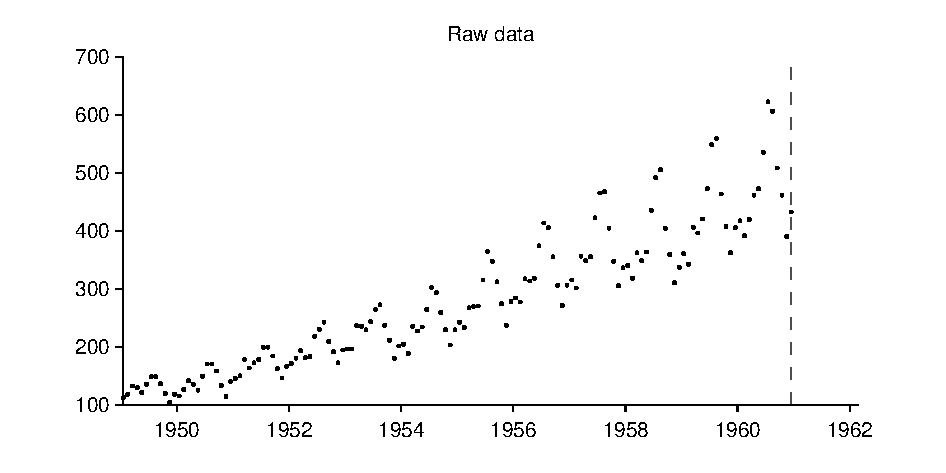
\includegraphics[width=\wmgd,height=\hmgd]{\mdrd/01-airline_raw_data} & 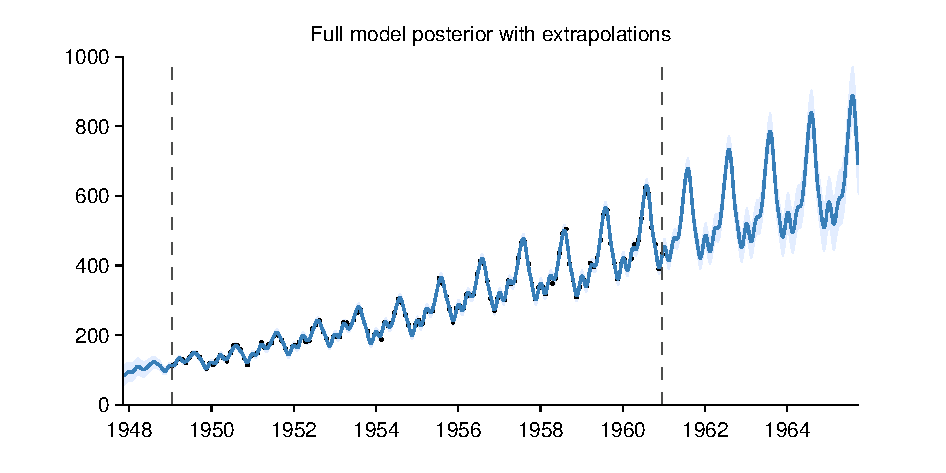
\includegraphics[width=\wmgd,height=\hmgd]{\mdrd/01-airline_all}
\end{tabular}
\caption{Raw data (left) and model posterior with extrapolation (right)}
\label{fig:rawandfit}
\end{figure}

The structure search algorithm has identified four additive components in the data.
The  first 2 additive components explain 99.3\% of the variation in the data as shown by the coefficient of determination ($R^2$) values in table~\ref{table:stats}.
After the first 3 components the cross validated mean absolute error (MAE) does not decrease by more than 0.1\%.
This suggests that subsequent terms are modelling very short term trends, uncorrelated noise or are artefacts of the model or search procedure.
Short summaries of the additive components are as follows:
\begin{itemize}

  \item A linearly increasing function. 

  \item An approximately periodic function with a period of 1.0 years and with linearly increasing amplitude. 

  \item A smooth function. 

  \item Uncorrelated noise with linearly increasing standard deviation. 

\end{itemize}

\begin{table}[htb]
\begin{center}
{\small
\begin{tabular}{|r|rrrrr|}
\hline
\bf{\#} & {$R^2$ (\%)} & {$\Delta R^2$ (\%)} & {Residual $R^2$ (\%)} & {Cross validated MAE} & Reduction in MAE (\%)\\
\hline
- & - & - & - & 280.30 & -\\

1 & 86.2 & 86.2 & 86.2 & 32.42 & 88.4\\

2 & 99.3 & 13.1 & 95.1 & 9.57 & 70.5\\

3 & 99.8 & 0.5 & 68.1 & 7.54 & 21.2\\

4 & 100.0 & 0.2 & 100.0 & 7.54 & 0.0\\

\hline
\end{tabular}
\caption{
Summary statistics for cumulative additive fits to the data.
The residual coefficient of determination ($R^2$) values are computed using the residuals from the previous fit as the target values; this measures how much of the residual variance is explained by each new component.
The mean absolute error (MAE) is calculated using 10 fold cross validation with a contiguous block design; this measures the ability of the model to interpolate and extrapolate over moderate distances.
The model is fit using the full data so the MAE values cannot be used reliably as an estimate of out-of-sample predictive performance.
}
\label{table:stats}
}
\end{center}
\end{table}

\section{Detailed discussion of additive components}

\subsection{Component 1 : A very smooth monotonically increasing function}

This function is very smooth and monotonically increasing.

This component explains 86.2\% of the total variance.
The addition of this component reduces the cross validated MAE by 88.4\% from 280.3 to 32.4.


\begin{figure}[H]
\newcommand{\wmgd}{0.5\columnwidth}
\newcommand{\hmgd}{3.0cm}
\newcommand{\mdrd}{figures/01-airline}
\newcommand{\mbm}{\hspace{-0.3cm}}
\begin{tabular}{cc}
\mbm 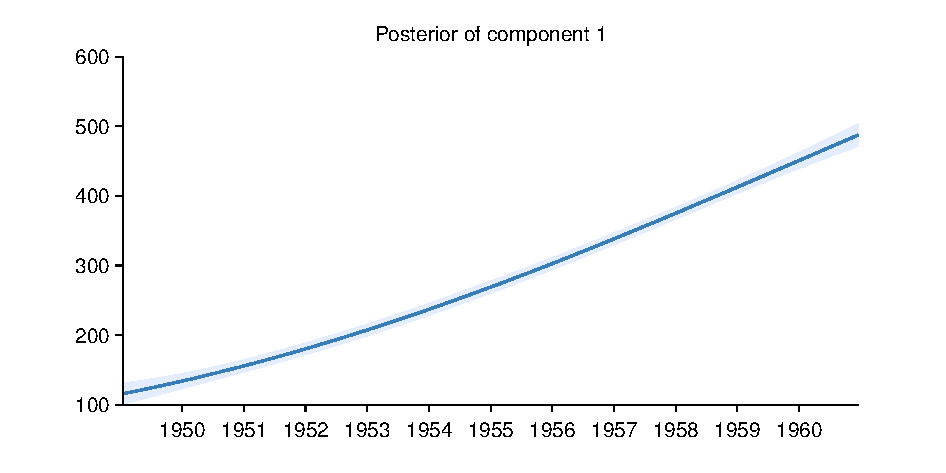
\includegraphics[width=\wmgd,height=\hmgd]{\mdrd/01-airline_1} & 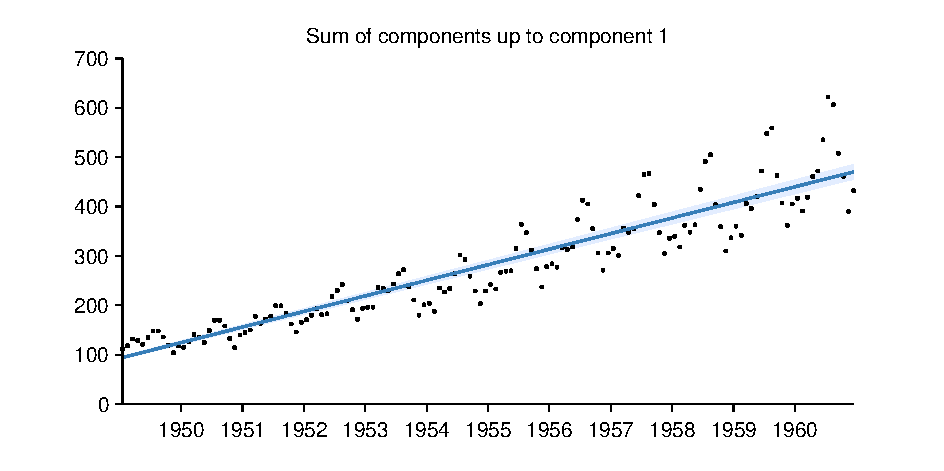
\includegraphics[width=\wmgd,height=\hmgd]{\mdrd/01-airline_1_cum}
\end{tabular}
\caption{Posterior of component 1 (left) and the posterior of the cumulative sum of components with data (right)}
\label{fig:comp1}
\end{figure}

\subsection{Component 2 : An approximately periodic function with a period of 1.0 years and with approximately linearly increasing amplitude}

This component is approximately periodic with a period of 1.0 years and varying amplitude.
Across periods the shape of this function varies very smoothly.
The amplitude of the function increases approximately linearly.
The shape of this function within each period has a typical lengthscale of 6.1 weeks.

This component explains 95.1\% of the residual variance; this increases the total variance explained from 86.2\% to 99.3\%.
The addition of this component reduces the cross validated MAE by 70.47\% from 32.42 to 9.57.


\begin{figure}[H]
\newcommand{\wmgd}{0.5\columnwidth}
\newcommand{\hmgd}{3.0cm}
\newcommand{\mdrd}{figures/01-airline}
\newcommand{\mbm}{\hspace{-0.3cm}}
\begin{tabular}{cc}
\mbm 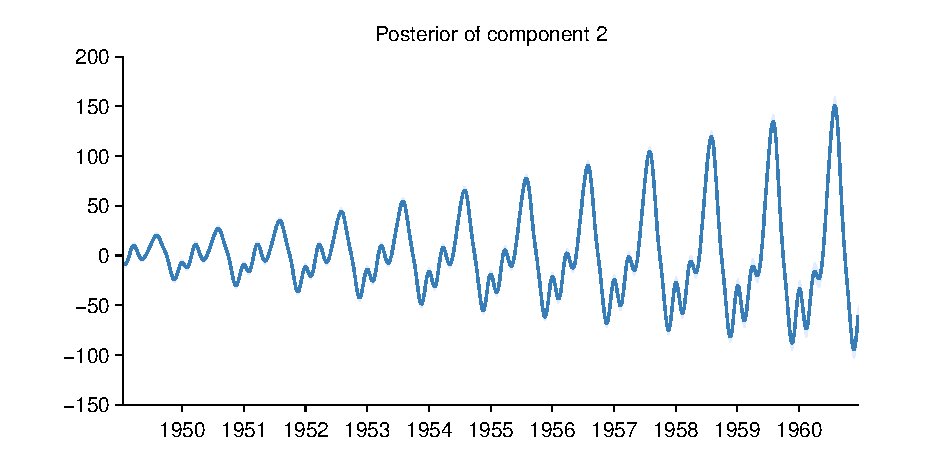
\includegraphics[width=\wmgd,height=\hmgd]{\mdrd/01-airline_2} & 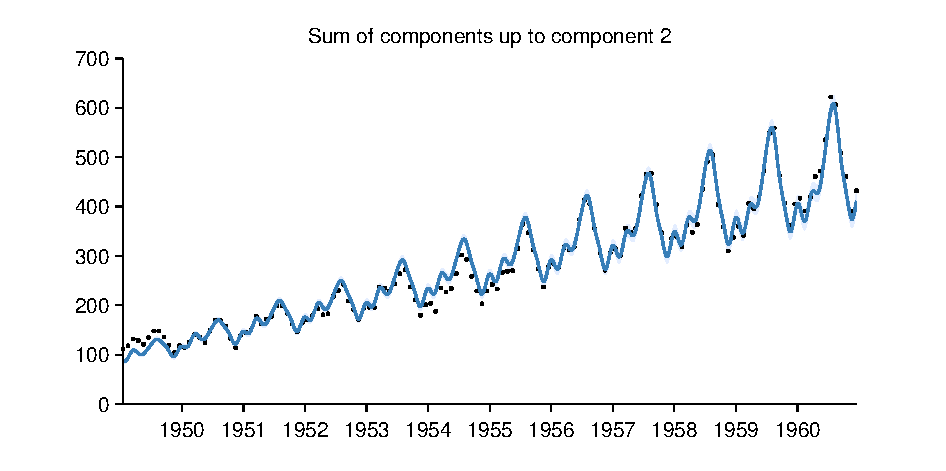
\includegraphics[width=\wmgd,height=\hmgd]{\mdrd/01-airline_2_cum}
\end{tabular}
\caption{Posterior of component 2 (left) and the posterior of the cumulative sum of components with data (right)}
\label{fig:comp2}
\end{figure}

\subsection{Component 3 : A smooth function}

This component is a smooth function with a typical lengthscale of 8.1 months.

This component explains 68.1\% of the residual variance; this increases the total variance explained from 99.3\% to 99.8\%.
The addition of this component reduces the cross validated MAE by 21.22\% from 9.57 to 7.54.


\begin{figure}[H]
\newcommand{\wmgd}{0.5\columnwidth}
\newcommand{\hmgd}{3.0cm}
\newcommand{\mdrd}{figures/01-airline}
\newcommand{\mbm}{\hspace{-0.3cm}}
\begin{tabular}{cc}
\mbm 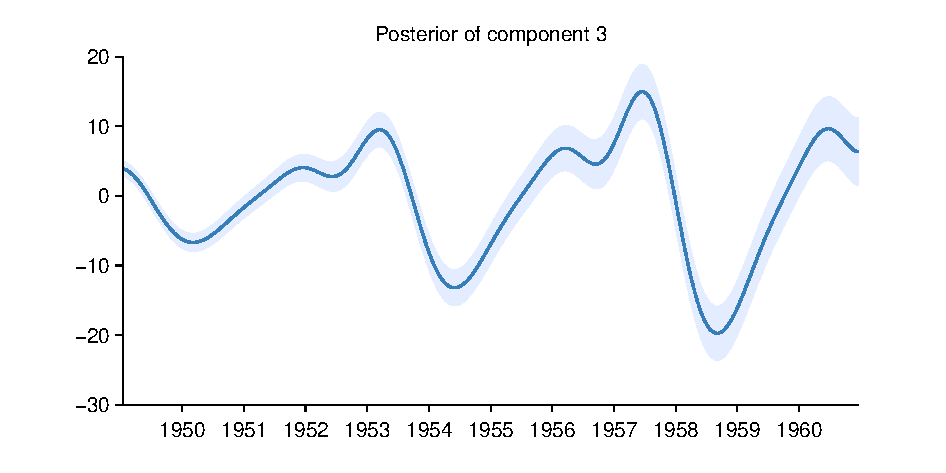
\includegraphics[width=\wmgd,height=\hmgd]{\mdrd/01-airline_3} & 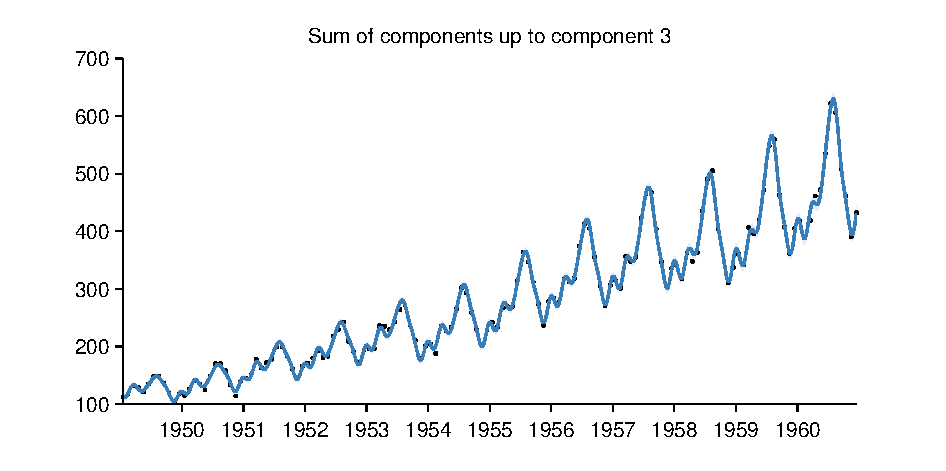
\includegraphics[width=\wmgd,height=\hmgd]{\mdrd/01-airline_3_cum}
\end{tabular}
\caption{Posterior of component 3 (left) and the posterior of the cumulative sum of components with data (right)}
\label{fig:comp3}
\end{figure}

\subsection{Component 4 : Uncorrelated noise with linearly increasing standard deviation}

This component models uncorrelated noise.
The standard deviation of the noise increases linearly.

This component explains 100.0\% of the residual variance; this increases the total variance explained from 99.8\% to 100.0\%.
The addition of this component reduces the cross validated MAE by 0.00\% from 7.54 to 7.54.
This component explains residual variance but does not improve MAE which suggests that this component describes very short term patterns, uncorrelated noise or is an artefact of the model or search procedure.

\begin{figure}[H]
\newcommand{\wmgd}{0.5\columnwidth}
\newcommand{\hmgd}{3.0cm}
\newcommand{\mdrd}{figures/01-airline}
\newcommand{\mbm}{\hspace{-0.3cm}}
\begin{tabular}{cc}
\mbm 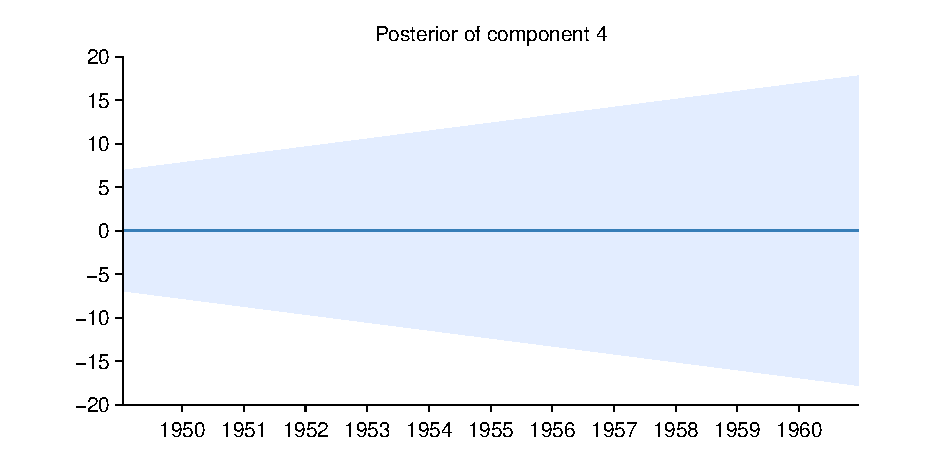
\includegraphics[width=\wmgd,height=\hmgd]{\mdrd/01-airline_4} & 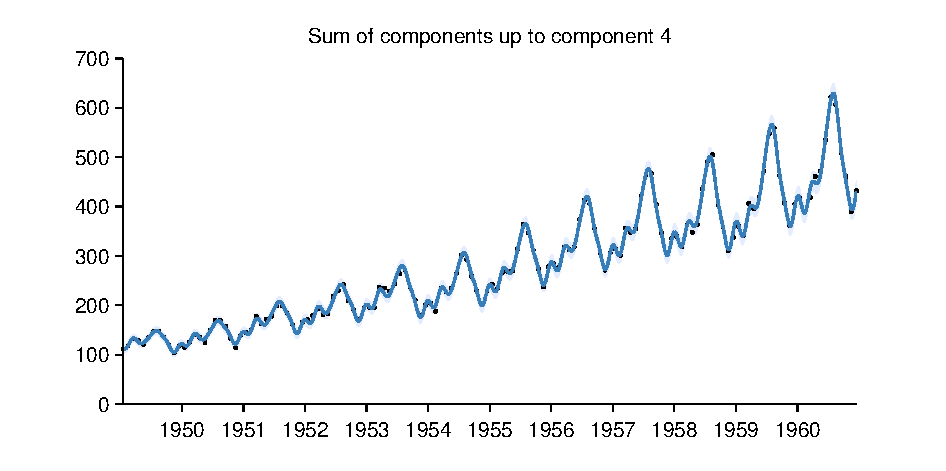
\includegraphics[width=\wmgd,height=\hmgd]{\mdrd/01-airline_4_cum}
\end{tabular}
\caption{Posterior of component 4 (left) and the posterior of the cumulative sum of components with data (right)}
\label{fig:comp4}
\end{figure}

\section{Extrapolation}

Summaries of the posterior distribution of the full model are shown in figure~\ref{fig:extrap}.
The plot on the left displays the mean of the posterior together with pointwise variance.
The plot on the right displays three random samples from the posterior.

\begin{figure}[H]
\newcommand{\wmgd}{0.5\columnwidth}
\newcommand{\hmgd}{3.0cm}
\newcommand{\mdrd}{figures/01-airline}
\newcommand{\mbm}{\hspace{-0.3cm}}
\begin{tabular}{cc}
\mbm 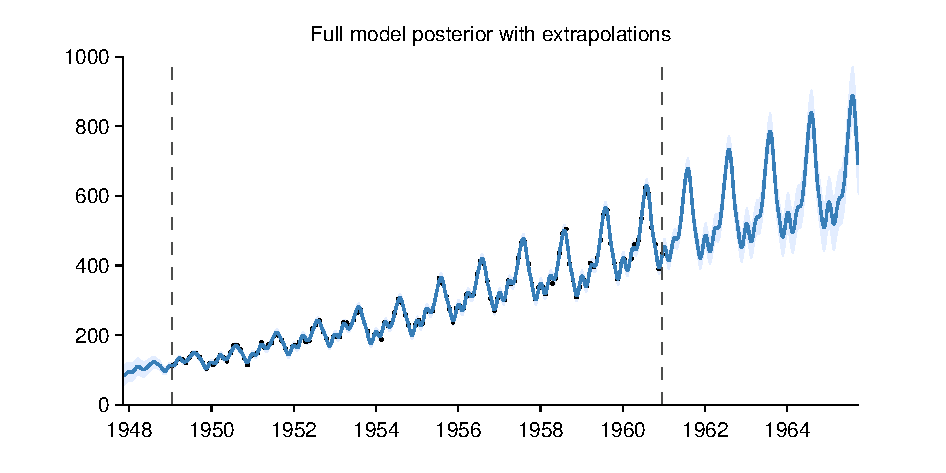
\includegraphics[width=\wmgd,height=\hmgd]{\mdrd/01-airline_all} & 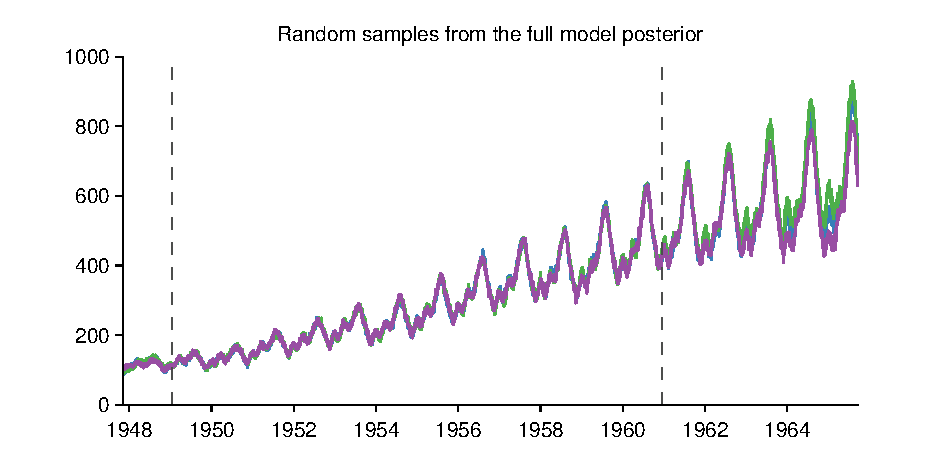
\includegraphics[width=\wmgd,height=\hmgd]{\mdrd/01-airline_all_sample}
\end{tabular}
\caption{Full model posterior. Mean and pointwise variance (left) and three random samples (right)}
\label{fig:extrap}
\end{figure}

\subsection{Component 1 : A very smooth monotonically increasing function}

Some discussion about extrapolation.

\begin{figure}[H]
\newcommand{\wmgd}{0.5\columnwidth}
\newcommand{\hmgd}{3.0cm}
\newcommand{\mdrd}{figures/01-airline}
\newcommand{\mbm}{\hspace{-0.3cm}}
\begin{tabular}{cc}
\mbm 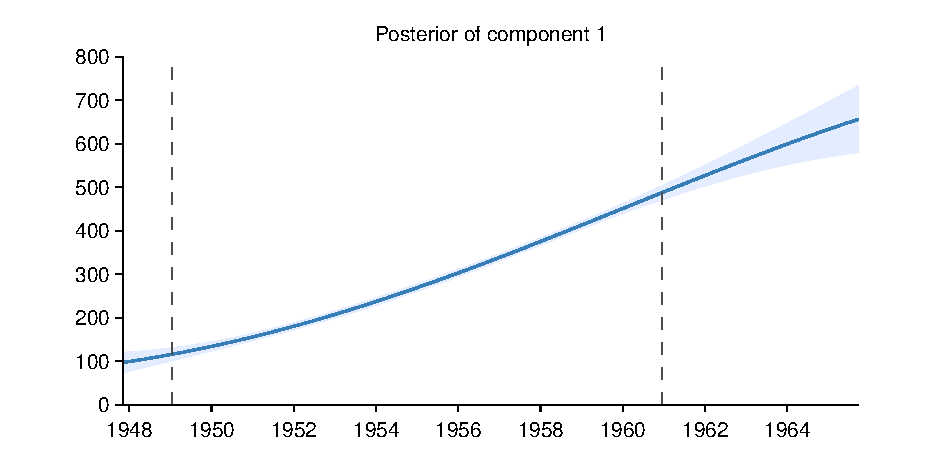
\includegraphics[width=\wmgd,height=\hmgd]{\mdrd/01-airline_1_extrap} & 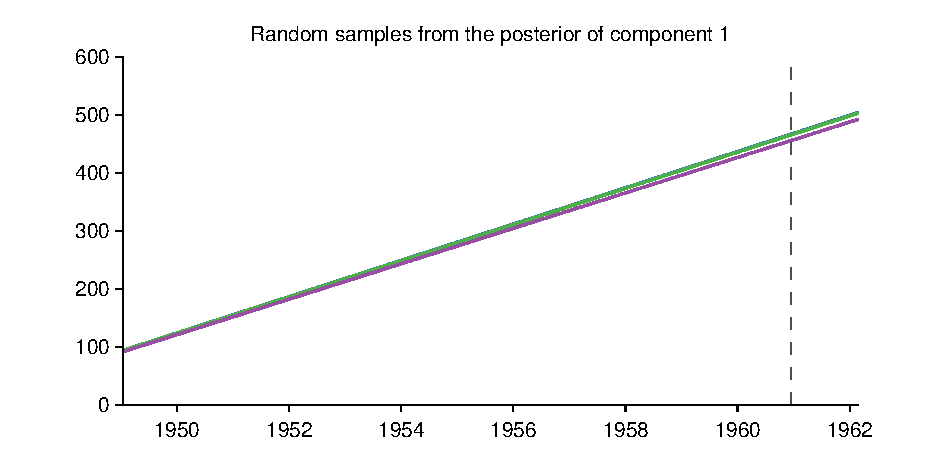
\includegraphics[width=\wmgd,height=\hmgd]{\mdrd/01-airline_1_sample} \\
\mbm 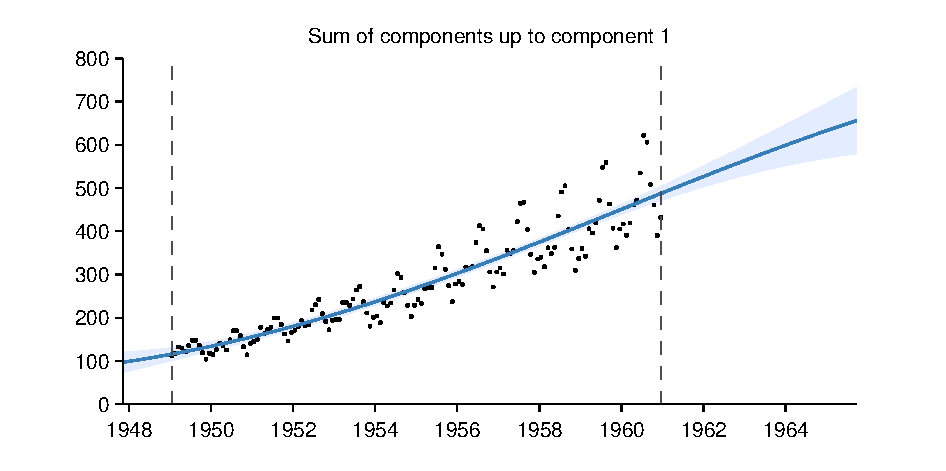
\includegraphics[width=\wmgd,height=\hmgd]{\mdrd/01-airline_1_cum_extrap} & 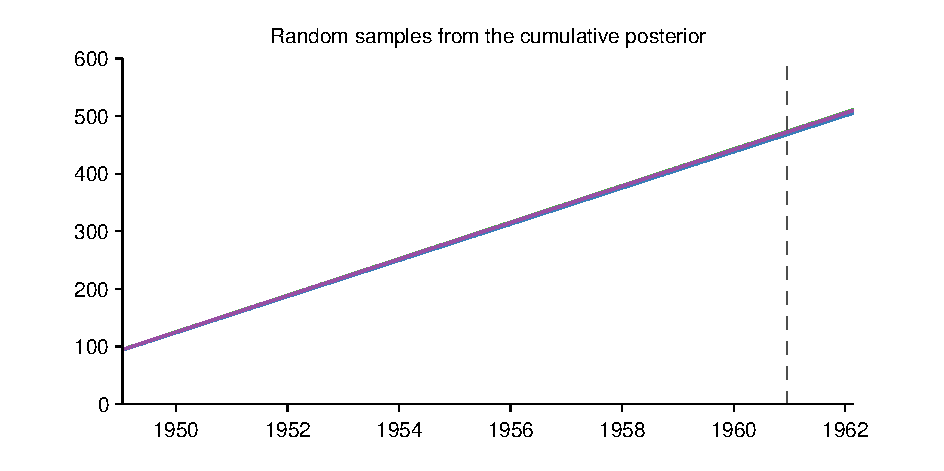
\includegraphics[width=\wmgd,height=\hmgd]{\mdrd/01-airline_1_cum_sample}
\end{tabular}
\caption{Posterior of component 1. Mean and pointwise variance (left) and three random samples from this distribution (right)}
\label{fig:extrap1}
\end{figure}

\subsection{Component 2 : An approximately periodic function with a period of 1.0 years and with approximately linearly increasing amplitude}

Some discussion about extrapolation.

\begin{figure}[H]
\newcommand{\wmgd}{0.5\columnwidth}
\newcommand{\hmgd}{3.0cm}
\newcommand{\mdrd}{figures/01-airline}
\newcommand{\mbm}{\hspace{-0.3cm}}
\begin{tabular}{cc}
\mbm 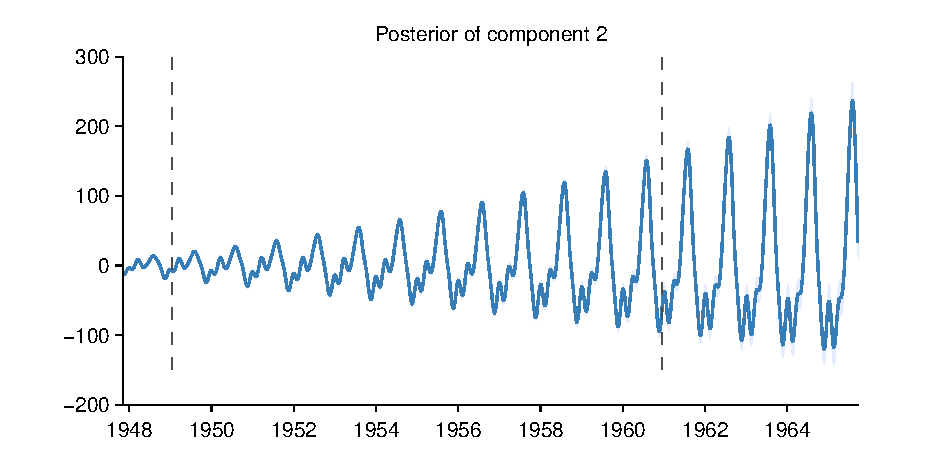
\includegraphics[width=\wmgd,height=\hmgd]{\mdrd/01-airline_2_extrap} & 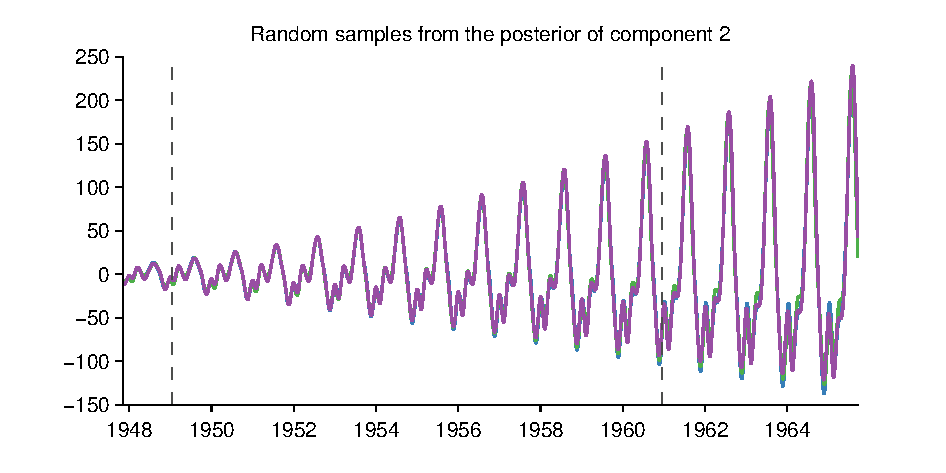
\includegraphics[width=\wmgd,height=\hmgd]{\mdrd/01-airline_2_sample} \\
\mbm 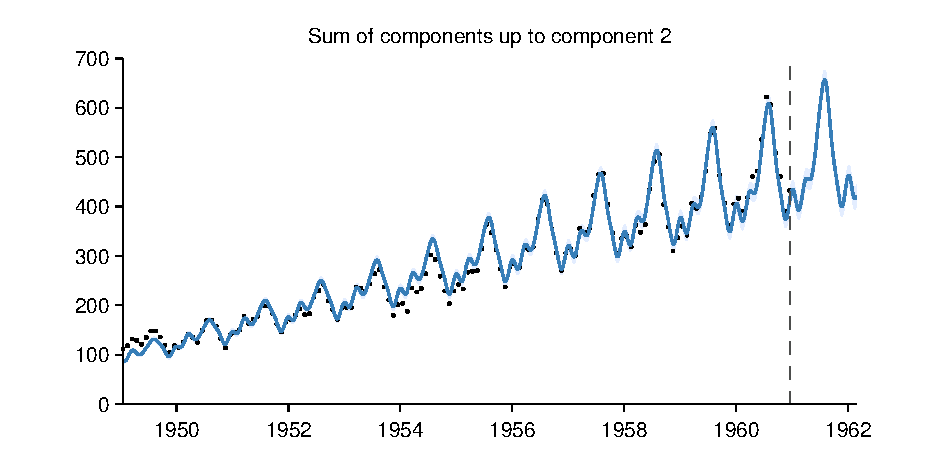
\includegraphics[width=\wmgd,height=\hmgd]{\mdrd/01-airline_2_cum_extrap} & 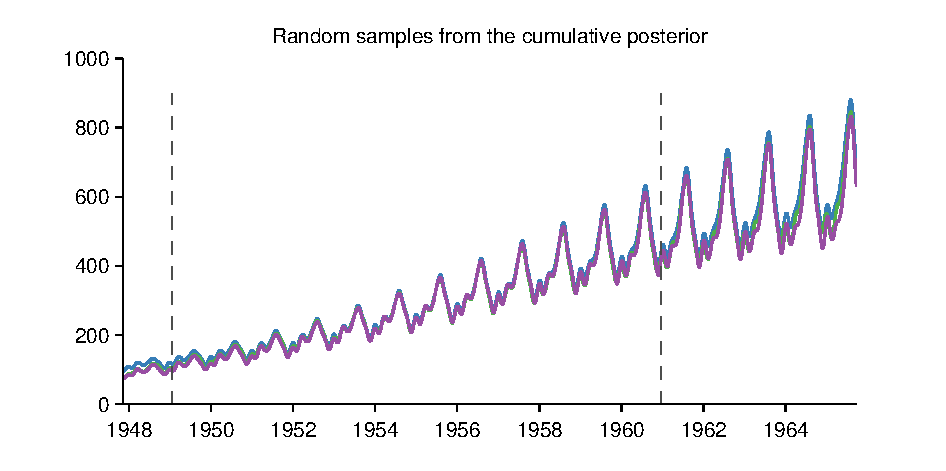
\includegraphics[width=\wmgd,height=\hmgd]{\mdrd/01-airline_2_cum_sample}
\end{tabular}
\caption{Posterior of component 2. Mean and pointwise variance (left) and three random samples from this distribution (right)}
\label{fig:extrap2}
\end{figure}

\subsection{Component 3 : A smooth function}

Some discussion about extrapolation.

\begin{figure}[H]
\newcommand{\wmgd}{0.5\columnwidth}
\newcommand{\hmgd}{3.0cm}
\newcommand{\mdrd}{figures/01-airline}
\newcommand{\mbm}{\hspace{-0.3cm}}
\begin{tabular}{cc}
\mbm 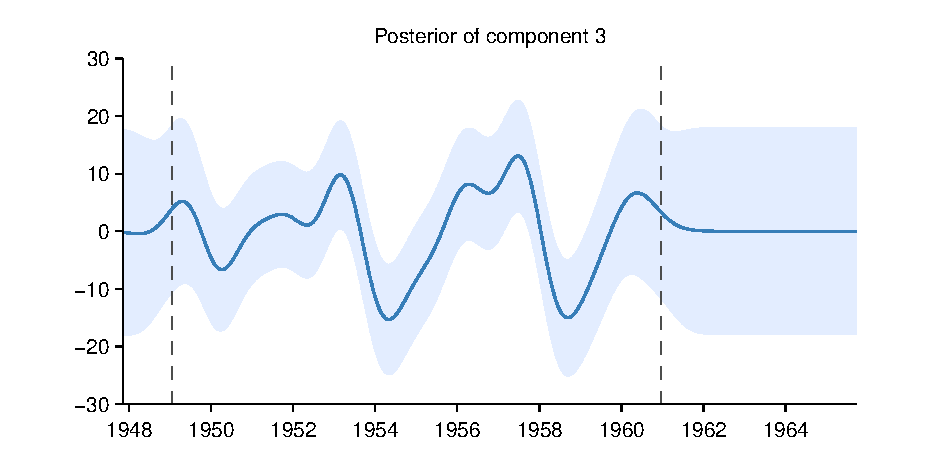
\includegraphics[width=\wmgd,height=\hmgd]{\mdrd/01-airline_3_extrap} & 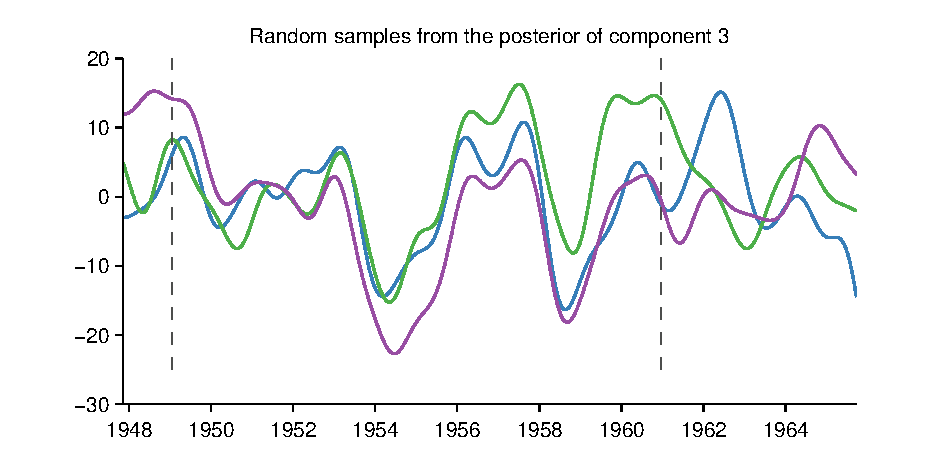
\includegraphics[width=\wmgd,height=\hmgd]{\mdrd/01-airline_3_sample} \\
\mbm 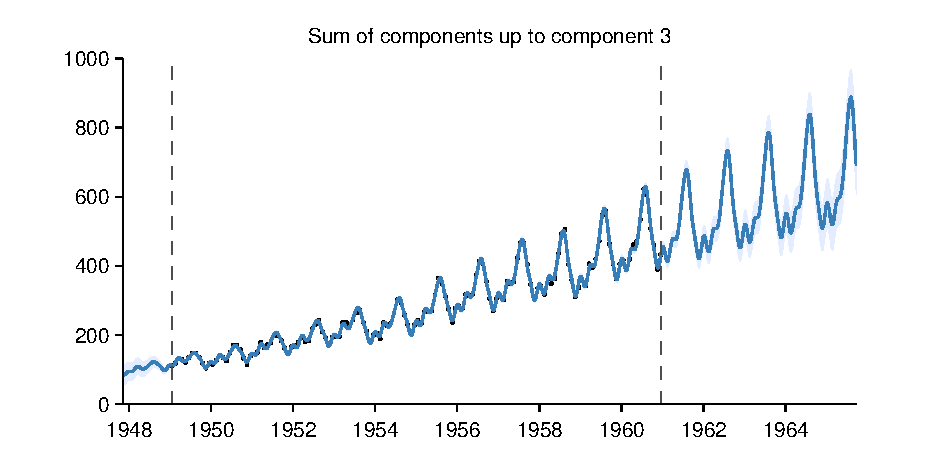
\includegraphics[width=\wmgd,height=\hmgd]{\mdrd/01-airline_3_cum_extrap} & 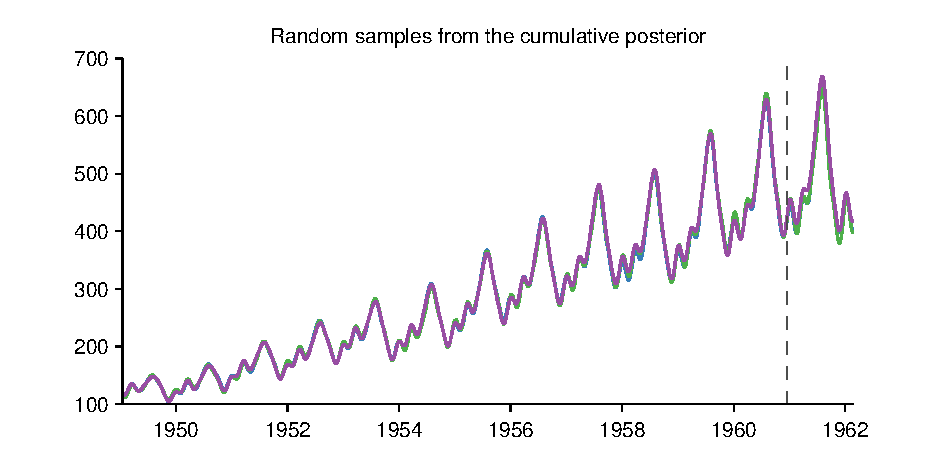
\includegraphics[width=\wmgd,height=\hmgd]{\mdrd/01-airline_3_cum_sample}
\end{tabular}
\caption{Posterior of component 3. Mean and pointwise variance (left) and three random samples from this distribution (right)}
\label{fig:extrap3}
\end{figure}

\subsection{Component 4 : Uncorrelated noise with linearly increasing standard deviation}

Some discussion about extrapolation.

\begin{figure}[H]
\newcommand{\wmgd}{0.5\columnwidth}
\newcommand{\hmgd}{3.0cm}
\newcommand{\mdrd}{figures/01-airline}
\newcommand{\mbm}{\hspace{-0.3cm}}
\begin{tabular}{cc}
\mbm 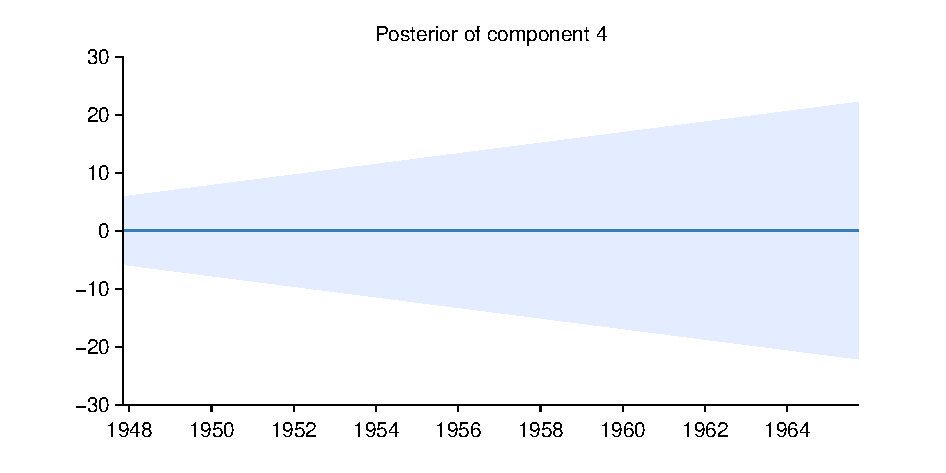
\includegraphics[width=\wmgd,height=\hmgd]{\mdrd/01-airline_4_extrap} & 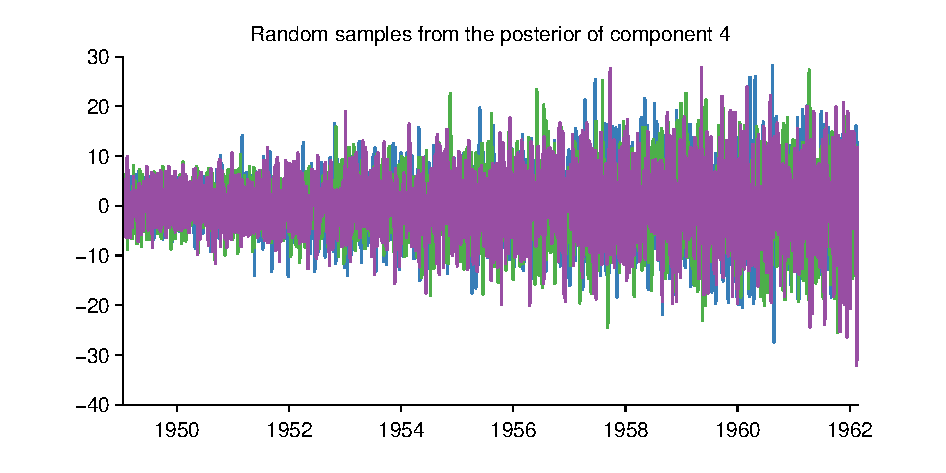
\includegraphics[width=\wmgd,height=\hmgd]{\mdrd/01-airline_4_sample} \\
\mbm 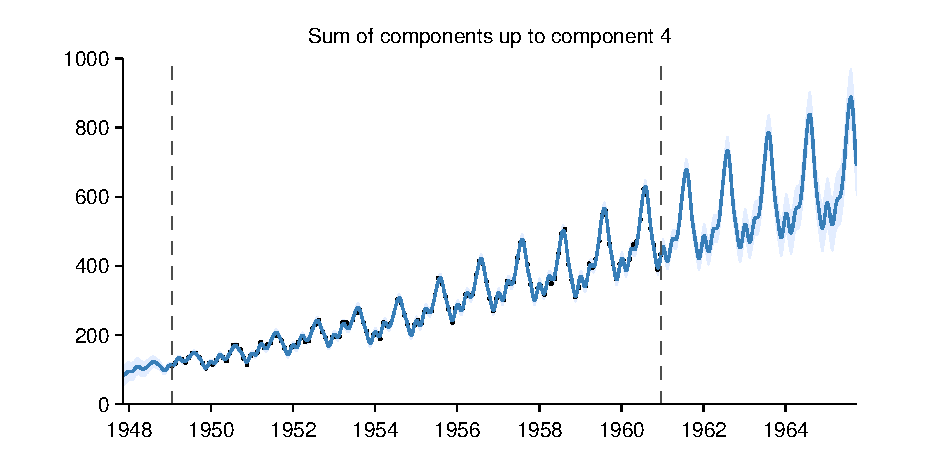
\includegraphics[width=\wmgd,height=\hmgd]{\mdrd/01-airline_4_cum_extrap} & 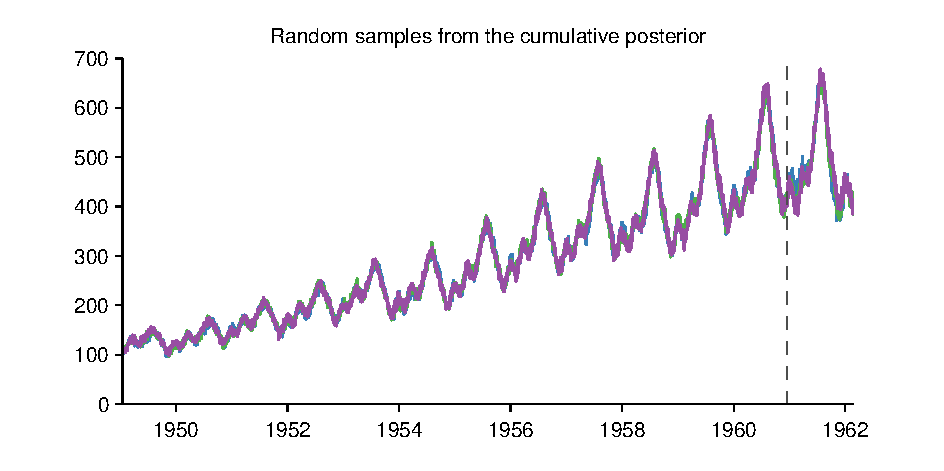
\includegraphics[width=\wmgd,height=\hmgd]{\mdrd/01-airline_4_cum_sample}
\end{tabular}
\caption{Posterior of component 4. Mean and pointwise variance (left) and three random samples from this distribution (right)}
\label{fig:extrap4}
\end{figure}

\end{document}
